\documentclass[a4paper,14pt]{extarticle}

\usepackage[utf8x]{inputenc}
\usepackage[T1,T2A]{fontenc}
\usepackage[russian]{babel}
\usepackage{hyperref}
\usepackage{indentfirst}
\usepackage{here}
\usepackage{array}
\usepackage{graphicx}
\usepackage{caption}
\usepackage{subcaption}
\usepackage{chngcntr}
\usepackage{amsmath}
\usepackage{amssymb}
\usepackage{pgfplots}
\usepackage{pgfplotstable}
\usepackage[left=2cm,right=2cm,top=2cm,bottom=2cm,bindingoffset=0cm]{geometry}
\usepackage{multicol}

\renewcommand{\le}{\ensuremath{\leqslant}}
\renewcommand{\leq}{\ensuremath{\leqslant}}
\renewcommand{\ge}{\ensuremath{\geqslant}}
\renewcommand{\geq}{\ensuremath{\geqslant}}
\renewcommand{\epsilon}{\ensuremath{\varepsilon}}
\renewcommand{\phi}{\ensuremath{\varphi}}

\counterwithin{figure}{section}
\counterwithin{equation}{section}
\counterwithin{table}{section}
\newcommand{\sign}[1][5cm]{\makebox[#1]{\hrulefill}} % Поля подписи и даты
\graphicspath{{pics/}} % Путь до папки с картинками
\captionsetup{justification=centering,margin=1cm}
\def\arraystretch{1.3}

\begin{document}

\begin{titlepage}
\begin{center}
	\textbf{Санкт-Петербургский Политехнический Университет \\Петра Великого}\\[0.3cm]
	\small Институт компьютерных наук и технологий \\[0.3cm]
	\small Кафедра компьютерных систем и программных технологий\\[4cm]
	
	\textbf{ОТЧЕТ}\\ \textbf{о лабораторной работе}\\[0.5cm]
	\textbf{<<Исследование частотных характеристик пассивных RC-цепей>>}\\[0.1cm]
	\textbf{Электротехника и Электроника}\\[10.5cm]
\end{center}

\begin{flushright}
	\begin{minipage}{0.60\textwidth}
		\begin{flushleft}
			\small \textbf{Работу выполнили студенты}\\[3mm]
			\small группа 23501/4 \hspace*{17mm} Дьячков В.В.\\[3mm]
			\small группа 23501/4 \hspace*{17mm} Ламтев А.Ю.\\[5mm]
			
			\small \textbf{Преподаватель}\\[5mm]
		 	\small \sign[3.5cm] \hspace*{8mm} к.т.н., доц. Кочетков Ю.Д.\\[0.5cm]
		\end{flushleft}
	\end{minipage}
\end{flushright}

\vfill

\begin{center}
	\small Санкт-Петербург\\
	\small \the\year
\end{center}
\end{titlepage}

\section{Цель работы}

Настройка и расчет масштабирующих устройств, постоянного и переменного токов с двумя и одним источником питания, источника тока, управляемого напряжением, алгебраического сумматора.

\section{Чертеж схемы исследуемого устройства}

\begin{figure}[H]
\begin{center}
	\begin{subfigure}[b]{0.3\textwidth}
		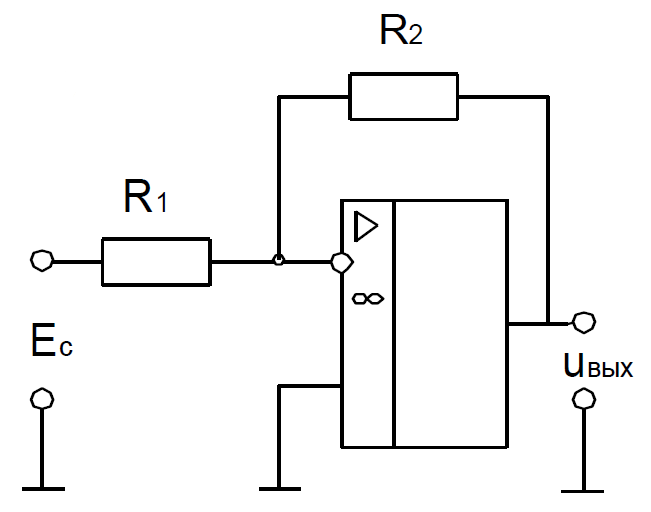
\includegraphics[scale=0.25]{first}
		\caption{Операционный усилитель с инверсией фазы}
	\end{subfigure}
	\begin{subfigure}[b]{0.3\textwidth}
		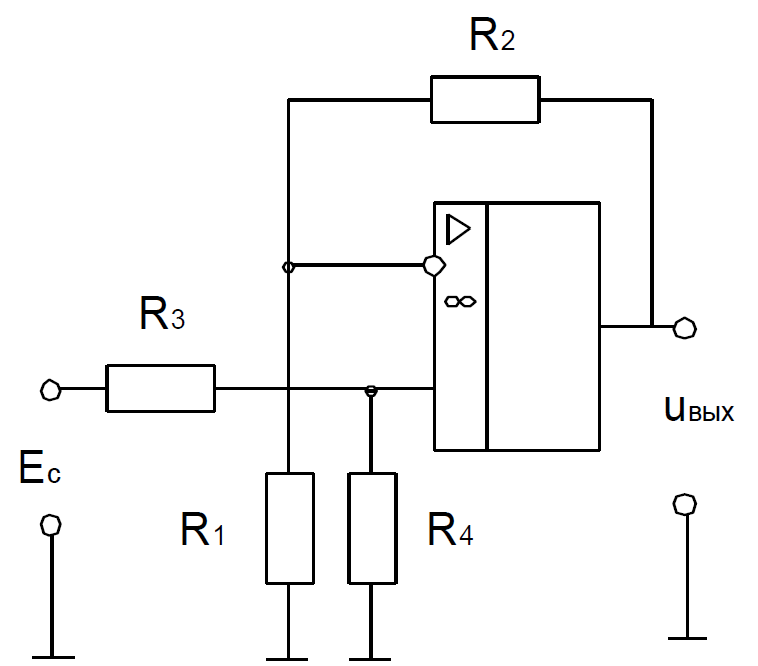
\includegraphics[scale=0.25]{second}
		\caption{Операционный усилитель без инверсии фазы}
	\end{subfigure}
	\begin{subfigure}[b]{0.3\textwidth}
		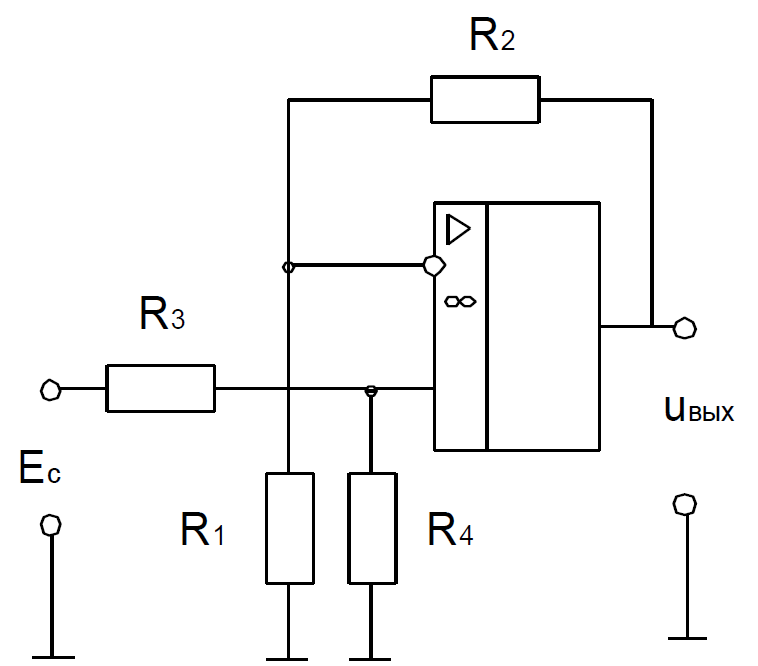
\includegraphics[scale=0.25]{second}
		\captionsetup{justification=centering}
		\caption{???}
	\end{subfigure}
	\caption{}
\end{center}
\end{figure}


\section{Исходные данные}

Операционный усилитель \verb+К140УД6+.

\begin{table}[H]
\begin{center}
	\caption{Исходные данные}
	\def\tabcolsep{50pt}
	\begin{tabular}{|c|c|c|c|c|c|c|c|c|c|}
		\hline
		$K$ &
		$f$, Гц &
		$i_\text{н}$, мА \\
		\hline
		1 &
		500 &
		0.5 \\
	    \hline	
	\end{tabular}
	\label{tabular:1}
\end{center}
\end{table}

\section{Теоретические расчёты}

\section{Экспериментально снятые зависимости}

В таблице \ref{tab:k_dc} и на рисунке \ref{tab:k_dc} приведена амплитудная характеристика усилителя $U_\text{вых} = f(e_c)$.

\begin{table}[H]
\begin{center}
	\caption{Зависимость напряжения $U_\text{вых}$ от $e_c$}
	\label{tab:k_dc}
	\def\tabcolsep{40pt}
	\def\arraystretch{1.2}
	\fontsize{13}{13}\selectfont
	\pgfplotstabletypeset[col sep=comma,
	    columns={e_c,u_out,k},
	    column type/.add={|c|}{},
	    columns/e_c/.style={fixed, precision=3, zerofill, column name={$e_c$, В}},
	    columns/u_out/.style={fixed, precision=3, zerofill, column name={$U_\text{вых}$, В}},
	    columns/k/.style={fixed, precision=2, zerofill, column name={$K$}},
	    every nth row={1}{before row=\hline},
	    every head row/.style={before row=\hline, after row=\hline},
	    every last row/.style={after row=\hline}
	   ]{data/k_dc.csv}
\end{center}
\end{table}

\begin{figure}[H]
\begin{center}
	\begin{tikzpicture} [every plot/.append style={thick}]
		\begin{axis}[
			height=0.4\textheight,
			width=0.9\textwidth,
			legend pos=north east,
			xlabel={$e_c$, В},
			ylabel={$U_\text{вых}$, В},
			xlabel near ticks,
			ylabel near ticks,
			xmin = -16,
			xmax = 16,
			ymin = -15,
			ymax = 15,
			grid=major
		]
		\addplot table[x=e_c,y=u_out,col sep=comma]{data/k_dc.csv};
%		\addplot table[x=e_c,y=u_out,col sep=comma]{data/ampl_theory.csv};
		\legend{Эксп., Teор.}
		\end{axis}
	\end{tikzpicture}
	\caption{Зависимость напряжения $U_\text{вых}$ от $e_c$}
	\label{fig:ampl}
\end{center}
\end{figure}

\section{Погрешности}

\section{Выводы}

Вычесленные уточнённые теоретические и полученные экспериментальные значения близки. Следовательно, формулы \ref{eq:r_in} -- \ref{eq:k_u0} могут быть использованы при расчетах.

\end{document}